\pagestyle{fancy}
\fancyhf{}
\fancyhead[R]{\texttt{kvant.mccme.ru}}
\renewcommand{\headrulewidth}{0pt}
\begin{center}
    {\LARGE\bfseries 38}
    \vspace{-0.5em}
    \rule{\textwidth}{0.2pt}
    {\textbf {задачник кванта}}
\end{center}





\begin{multicols}{2}

\raggedleft
клеток \(mn\)/2 костями домино (прямоугольниками 1 x 2 клетки, разуммеется; 
мы считаем одно из чисел \(m\) и \(n\) чётным).\newline
a) Докажите, что \(p_{2,n} = f_{n}\)- последовательность, задаваемая соотношением
\(f_{n + 1} = f_{n} + f_{n - 1}\); \(f_1 = 1\), \(f_2 = 2\)(последовательность Фибоначчи).\newline 
Б)* Докажите, что (для чётных \(n\)) верны оценки 
\[(3/2)^{n^{2}/2} < p_{n, n} < 2^{n^{2}/2}\]

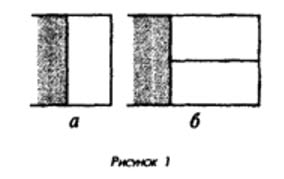
\includegraphics{/home/cun/Documents/LatexLab/photos/photo_2024-12-03_02-54-34.jpg}

\begin{center}
    \begin{tabular}{|p{4cm}|p{4cm}|}
        \hline
        \centering n\arraybackslash & \centering F\textsubscript{n}\arraybackslash \\ [0.5ex]
        \hline
        \centering 1\arraybackslash & \centering 1 \arraybackslash \\
        \centering 2\arraybackslash & \centering 2 \arraybackslash \\
        \centering 3\arraybackslash & \centering 3 \arraybackslash \\
        \centering 4\arraybackslash & \centering 5 \arraybackslash \\
        \centering 5\arraybackslash & \centering 8 \arraybackslash \\
        \centering 6\arraybackslash & \centering 1 3 \arraybackslash \\
        \centering 7\arraybackslash & \centering 2 1 \arraybackslash \\
        \centering 8\arraybackslash & \centering 3 4 \arraybackslash \\
        \centering 9\arraybackslash & \centering 5 5 \arraybackslash \\
        \centering 1 0\arraybackslash & \centering 8 9 \arraybackslash \\
        \centering \arraybackslash & \centering  \arraybackslash \\
        \centering ...\arraybackslash & \centering ... \arraybackslash \\
        \hline
    \end{tabular}
\end{center}


\columnbreak

\raggedright 
прямоугольника 2\(n\) можно добавить справа вертикальные домино, к любому покрытию
прямоугольника 2(\(n\) - 1) - два горизонтальных домино, и этим способом получаются по разу
все покрытия прямоугольника 2(\(n\) + 1). Отсюда \(f_{n + 1} = f_{n} + f_{n - 1}\). Равенства \(f_{1} = 1\)
, \(f_{2} = 2\) очевидны. Несколько следующих значений \(f_{n}\) приведены в таблице на полях. \newline
Числа этой последовательности - числа Фибоначчи - встречаются в самых разнообразных задачах комбинаторики
, геометрии, анализа. Для них можно написать явные формулы, выразив \(f_{n}\) в виде суммы двух
геометрических прогрессий:
    \[f_{n} = b_{1}q_{1}^{n} + b_{2}q_{2}^{n}\]
где \(q_{1}\), \(q_{2}\) - корни уравнения \(q^{2} = q + 1\)(т.е \(q_{i} = (1 \pm \sqrt{5}) / 2\)) a \(b_{i}\)
определяются начальными условиями \(f_{0} = f_{1} = 1\); в результате получаем \textit{формулу} Бинэ:
    \[f_{n} = (q_{1}^{n + 1} - q_{2}^{n + 1}) / \sqrt{5}\]
Поскольку \(|q_{2}| < 1\), при болиших \(n\) получаем \(f_{n} \approx B q_{1}^{n}\), где \(q_{1} = (1 + \sqrt{5}) / 2 \approx 1,61803...\);
\(B\) - константа,
    \[B = (1 + \sqrt{5}) / (2\sqrt{5})\]
Для решения задачи Б) удобно использовать оценку \(f_{n} > (3/2)^{n}\), верную при \(n \geq 5\). Её легко доказать
по индукции: \(f_{5} = 8 > (3/2)^{5} = 243 / 32\), \(f_{6} = 13 > (3/2)^{6} = 729 / 64\);
если \(f_{n - 1} > (3/2)^{n - 1}\) и \(f_{n} > (3/2)^{n}\), то \(f_{n + 1} = f_{n} + f_{n - 1} > (3/2)^{n - 1}(3/2 + 1) > (3/2)^{n + 1}\)
, поскольку \((3/2) + 1 = 5/2 > 9/4\).\newline
В задаче Б) левое неравенство (оценку снизу) для \(n = 4\) можно проверить непосредственно: \(p_{4,4} = 36\)(это - \(25 = 5.5\)
покрытий двух горизонтальных прямоугольников \(2 x 4\), и ещё 11 покрытий, а \((3/2)^{8} < 32 < 36\), поскольку \(3^{5} < 2^{8}\), \(3^{3} < 2^{5}\).\\
Для \(n \geq 6\) оценку снизу можно получить, рассмотреть лишь покрытия \(n/2\) горизонтальных полосок \(2n\) клеток:
поскольку \(f_{n} > (3/2)^{n}\), то
    \[p_{n, n} > (f_{n})^{n/2} > (3/2)^{n^{2}/2}\].


\end{multicols}